%!TEX root = ../../msc17-game-book.tex


\phChapterWorksheet{Which Witch?}{Main Puzzle 1}

Grendel the Witch is doing what witches do: brewing potions!

In order to work efficiently, Grendel wants to use three cauldrons at
the same time. Viewed from the top-down, each cauldron is perfectly
circular, with a radius of \(3\) feet.

\begin{center}
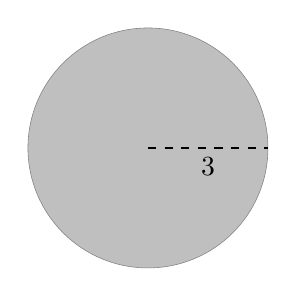
\begin{tikzpicture}[x=0.2in,y=0.2in]
  \draw[color=gray,very thin,fill=lightgray] (0,0) circle (3);
  \draw[dashed] (0,0) -- node[below] {3} (3,0);
\end{tikzpicture}
\end{center}

In order to stir each postion successfully, Grendel must be equally close
to all three cauldrons used.
\textbf{How can Grendel position the cauldrons so that she's as close as
possible to all three? How far would she be from the center of
each cauldron in this configuration?} She's a frail old thing, so don't
be afraid to squeeze her into a small space if necessary...

By the way,
some of Grendel's \textit{mathemagics} may help here. She has a feeling
that the following triangle is important to this particular puzzle.
It is drawn below such that the shortest side has length \(1\), but you
may need to scale things a bit...


\begin{center}
\begin{tikzpicture}[x=1in,y=1in]
  \draw (0,0) -- node[below] {1}
        (1,0) -- node[above right] {2}
        ($(0,{sqrt(3)})$) -- node[left] {\(\sqrt3\)}
        (0,0);
  \draw (0,0.1) -- (0.1,0.1) -- (0.1,0);
  \node at (0.13, 1.25) {\small\(30^\circ\)};
  \node at (0.8, 0.1) {\small\(60^\circ\)};
\end{tikzpicture}
\end{center}
